 \documentclass{article}
\usepackage[utf8]{inputenc}
\usepackage[a4paper, total={7in, 10in}]{geometry}
\usepackage{braket}
\usepackage{xcolor}
\usepackage{amsmath}
\usepackage{amssymb}
\usepackage{amsfonts}
\usepackage{graphicx}
\usepackage{svg}
\usepackage{float}
\usepackage{tikz}
\usepackage[ruled,vlined]{algorithm2e}
\usepackage{multicol}
\usepackage[backend=biber,style=alphabetic,sorting=ynt]{biblatex}
\usepackage{xcolor}
%\addbibresource{sample.bib} %Import the bibliography file

\newcommand{\commentt}[1]{\textcolor{blue}{ \textbf{[COMMENT]} #1}}
\newcommand{\ctt}[1]{\commentt{#1}}
\newcommand{\prb}[1]{ \mathbf{Pr} \left[ {#1} \right]}
\newcommand{\onotation}[1]{\(\mathcal{O} \left( {#1}  \right) \)}
\newcommand{\ona}[1]{\onotation{#1}}
\newcommand{\PSI}{{\ket{\psi}}}
\newcommand{\LESn}{\ket{\psi_n}}
\newcommand{\LESa}{\ket{\phi_n}}
\newcommand{\LESs}{\frac{1}{\sqrt{n}}\sum_{i}{\ket{\left(0^{i}10^{n-i}\right)^{n}}}}
\newcommand{\Hn}{\mathcal{H}_{n}}
\newcommand{\Ep}{\frac{1}{\sqrt{2^n}}\sum^{2^n}_{x}{ \ket{xx}}}
\newcommand{\HON}{\ket{\psi_{\text{honest}}}}
\newcommand{\Lemma}{\paragraph{Lemma.}}


\setlength{\columnsep}{0.6cm}

\newcommand{\Gz}{ G_{z}^{\delta} } 

\begin{document}

\title{Quantum LTC With Positive Rate}
\author{David Ponarovsky}
\maketitle
\begin{multicols*}{2}
\newcommand{ \Hw }{ \delta\Delta -\Delta^{\frac{1}{2}-\varepsilon}/\delta  }
	\newcommand{ \Nw }{ \Delta^{\frac{3}{2}-\varepsilon}} 
	  \newcommand{ \Gu } { \Gamma^{\cup} }
	  \newcommand{ \Guq } { \Gamma^{\cup, \square} }

    	\newcommand{ \Gsa } {\Gamma_{\square_{1}} }
	\newcommand{ \Gsb } {\Gamma_{\square_{2}} }
        \newcommand{ \Aa } { C_{A_{1}}}  
	\newcommand{ \Ab } { C_{A_{2}}}
	\newcommand{ \Ac } { C_{A_{3}}}
	\newcommand{ \Aab } { \Aa \otimes \Ab } 
	\newcommand{ \Aac } { \Aa \otimes \Ac }
	\newcommand{ \Aabc } { \Aa \otimes \Ab \otimes \Ac }
	\newcommand{ \Aabp } { \Aa^{\perp} \otimes \Ab^{\perp} } 
	\newcommand{ \Aacp } { \Aa^{\perp} \otimes \Ac^{\perp} }
	\newcommand{ \Aabcp } { \Aa^{\perp} \otimes \Ab^{\perp} \otimes \Ac^{\perp} }
	\newcommand{ \Aabpp } { \left( \Aabp \right)^\perp } 
	\newcommand{ \Aacpp } { \left( \Aacp \right)^\perp }
	\newcommand{ \Aabcpp } { \left( \Aabcp \right)^\perp }
	\newcommand{ \YY } {  y_{1}y_{2}^{\top} }
	\newcommand{ \ZZ } {  z_{1}z_{2}^{\top} } 
	\newcommand{ \TT } { \tilde{\tau} } 


  \paragraph{preamble.} preamble.  
  \begin{figure}[H]
            %\label{fig:square}
            \begin{center}
            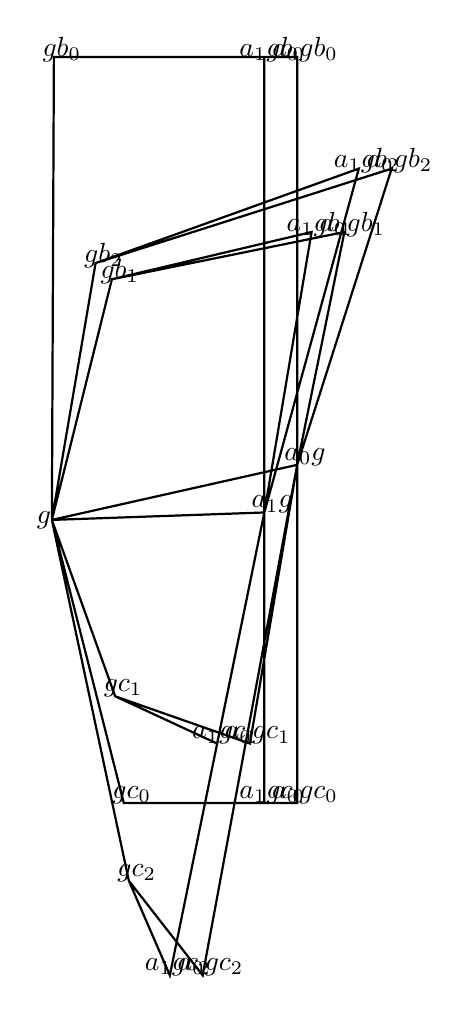
\begin{tikzpicture}
            \draw[thick](0,0)(0,0) -- (0.025676393503967,5.878120908798526) -- (3.115352492751059,5.878120908798526) -- (3.115352492751059,0.6995273259415428) -- (0,0)
(0,0) -- (0.7623292321810113,3.0563961653429024) -- (3.7153524927510593,3.6563961653429025) -- (3.115352492751059,0.6995273259415428) -- (0,0)
(0,0) -- (0.5553563500378105,3.261678910564688) -- (4.315352492751059,4.461678910564688) -- (3.115352492751059,0.6995273259415428) -- (0,0)
(0,0) -- (0.025676393503967,5.878120908798526) -- (2.6983087870148657,5.878120908798526) -- (2.6983087870148657,0.09437838498546348) -- (0,0)
(0,0) -- (0.7623292321810113,3.0563961653429024) -- (3.2983087870148657,3.6563961653429025) -- (2.6983087870148657,0.09437838498546348) -- (0,0)
(0,0) -- (0.5553563500378105,3.261678910564688) -- (3.898308787014866,4.461678910564688) -- (2.6983087870148657,0.09437838498546348) -- (0,0)
(0,0) -- (0.9133137130783713,-3.594636783146492) -- (3.115352492751059,-3.594636783146492) -- (3.115352492751059,0.6995273259415428) -- (0,0)
(0,0) -- (0.8041312830260496,-2.240056853360265) -- (2.515352492751059,-2.8400568533602653) -- (3.115352492751059,0.6995273259415428) -- (0,0)
(0,0) -- (0.9779705686238185,-4.583428054182538) -- (1.9153524927510592,-5.783428054182538) -- (3.115352492751059,0.6995273259415428) -- (0,0)
(0,0) -- (0.9133137130783713,-3.594636783146492) -- (2.6983087870148657,-3.594636783146492) -- (2.6983087870148657,0.09437838498546348) -- (0,0)
(0,0) -- (0.8041312830260496,-2.240056853360265) -- (2.0983087870148656,-2.8400568533602653) -- (2.6983087870148657,0.09437838498546348) -- (0,0)
(0,0) -- (0.9779705686238185,-4.583428054182538) -- (1.4983087870148657,-5.783428054182538) -- (2.6983087870148657,0.09437838498546348) -- (0,0)
;
\node at (3.2153524927510593,5.978120908798526) {$ a_{ 0  } gb_{ 0 } $};
\node at (3.8153524927510594,3.7563961653429025) {$ a_{ 0  } gb_{ 1 } $};
\node at (4.415352492751059,4.561678910564687) {$ a_{ 0  } gb_{ 2 } $};
\node at (2.7983087870148657,5.978120908798526) {$ a_{ 1  } gb_{ 0 } $};
\node at (3.398308787014866,3.7563961653429025) {$ a_{ 1  } gb_{ 1 } $};
\node at (3.998308787014866,4.561678910564687) {$ a_{ 1  } gb_{ 2 } $};
\node at (3.2153524927510593,-3.494636783146492) {$ a_{ 0  } gc_{ 0 } $};
\node at (2.615352492751059,-2.740056853360265) {$ a_{ 0  } gc_{ 1 } $};
\node at (2.015352492751059,-5.683428054182539) {$ a_{ 0  } gc_{ 2 } $};
\node at (2.7983087870148657,-3.494636783146492) {$ a_{ 1  } gc_{ 0 } $};
\node at (2.1983087870148657,-2.740056853360265) {$ a_{ 1  } gc_{ 1 } $};
\node at (1.5983087870148658,-5.683428054182539) {$ a_{ 1  } gc_{ 2 } $};
\node at (-0.1,0) {$ g $};
\node at (3.2153524927510593,0.7995273259415427) {$ a_{ 0 }g $};
\node at (2.7983087870148657,0.1943783849854635) {$ a_{ 1 }g $};
\node at (0.125676393503967,5.978120908798526) {$ gb_{ 0 } $};
\node at (0.8623292321810113,3.1563961653429025) {$ gb_{ 1 } $};
\node at (0.6553563500378105,3.361678910564688) {$ gb_{ 2 } $};
\node at (1.0133137130783714,-3.494636783146492) {$ gc_{ 0 } $};
\node at (0.9041312830260496,-2.140056853360265) {$ gc_{ 1 } $};
\node at (1.0779705686238186,-4.483428054182538) {$ gc_{ 2 } $};

            \end{tikzpicture}
            \end{center}
            \caption{Square of the complex, with edges $(g,ag), (agb, gb) \in E_A,
            (g,gb), (agb, ag) \in E_B.$ \label{fig:square}
            }
            \end{figure}
 \begin{figure}[H]
            %\label{fig:square}
            \begin{center}
            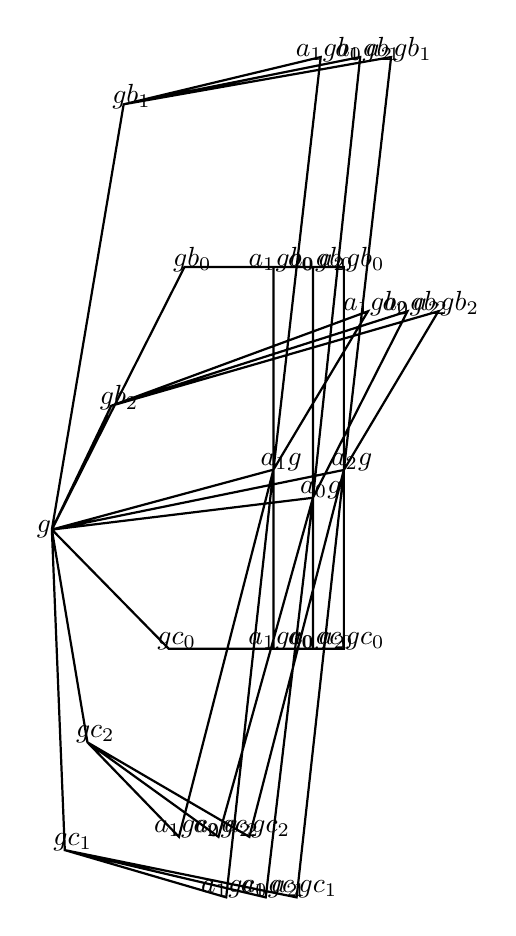
\begin{tikzpicture}
            \draw[thick](0,0)(0,0) -- (1.6845596083837637,3.3353499129341433) -- (3.315837025762871,3.3353499129341433) -- (3.315837025762871,0.4039617019549792) -- (0,0)
(0,0) -- (0.9117682796319366,5.4009135845475384) -- (3.915837025762871,6.000913584547538) -- (3.315837025762871,0.4039617019549792) -- (0,0)
(0,0) -- (0.7531757427481229,1.5719008510559127) -- (4.515837025762871,2.7719008510559124) -- (3.315837025762871,0.4039617019549792) -- (0,0)
(0,0) -- (1.6845596083837637,3.3353499129341433) -- (2.8138108386950824,3.3353499129341433) -- (2.8138108386950824,0.7610412741353239) -- (0,0)
(0,0) -- (0.9117682796319366,5.4009135845475384) -- (3.4138108386950825,6.000913584547538) -- (2.8138108386950824,0.7610412741353239) -- (0,0)
(0,0) -- (0.7531757427481229,1.5719008510559127) -- (4.013810838695083,2.7719008510559124) -- (2.8138108386950824,0.7610412741353239) -- (0,0)
(0,0) -- (1.6845596083837637,3.3353499129341433) -- (3.7082175147764236,3.3353499129341433) -- (3.7082175147764236,0.7571973212505595) -- (0,0)
(0,0) -- (0.9117682796319366,5.4009135845475384) -- (4.308217514776423,6.000913584547538) -- (3.7082175147764236,0.7571973212505595) -- (0,0)
(0,0) -- (0.7531757427481229,1.5719008510559127) -- (4.908217514776424,2.7719008510559124) -- (3.7082175147764236,0.7571973212505595) -- (0,0)
(0,0) -- (1.4844780163689955,-1.5135453154950227) -- (3.315837025762871,-1.5135453154950227) -- (3.315837025762871,0.4039617019549792) -- (0,0)
(0,0) -- (0.16419252697023135,-4.07067163772269) -- (2.715837025762871,-4.670671637722689) -- (3.315837025762871,0.4039617019549792) -- (0,0)
(0,0) -- (0.4518757697623754,-2.702037788103539) -- (2.115837025762871,-3.902037788103539) -- (3.315837025762871,0.4039617019549792) -- (0,0)
(0,0) -- (1.4844780163689955,-1.5135453154950227) -- (2.8138108386950824,-1.5135453154950227) -- (2.8138108386950824,0.7610412741353239) -- (0,0)
(0,0) -- (0.16419252697023135,-4.07067163772269) -- (2.2138108386950823,-4.670671637722689) -- (2.8138108386950824,0.7610412741353239) -- (0,0)
(0,0) -- (0.4518757697623754,-2.702037788103539) -- (1.6138108386950825,-3.902037788103539) -- (2.8138108386950824,0.7610412741353239) -- (0,0)
(0,0) -- (1.4844780163689955,-1.5135453154950227) -- (3.7082175147764236,-1.5135453154950227) -- (3.7082175147764236,0.7571973212505595) -- (0,0)
(0,0) -- (0.16419252697023135,-4.07067163772269) -- (3.1082175147764235,-4.670671637722689) -- (3.7082175147764236,0.7571973212505595) -- (0,0)
(0,0) -- (0.4518757697623754,-2.702037788103539) -- (2.5082175147764234,-3.902037788103539) -- (3.7082175147764236,0.7571973212505595) -- (0,0)
;
\node at (3.415837025762871,3.4353499129341434) {$ a_{ 0  } gb_{ 0 } $};
\node at (4.015837025762871,6.100913584547538) {$ a_{ 0  } gb_{ 1 } $};
\node at (4.615837025762871,2.8719008510559125) {$ a_{ 0  } gb_{ 2 } $};
\node at (2.9138108386950825,3.4353499129341434) {$ a_{ 1  } gb_{ 0 } $};
\node at (3.5138108386950826,6.100913584547538) {$ a_{ 1  } gb_{ 1 } $};
\node at (4.113810838695082,2.8719008510559125) {$ a_{ 1  } gb_{ 2 } $};
\node at (3.8082175147764237,3.4353499129341434) {$ a_{ 2  } gb_{ 0 } $};
\node at (4.408217514776423,6.100913584547538) {$ a_{ 2  } gb_{ 1 } $};
\node at (5.008217514776423,2.8719008510559125) {$ a_{ 2  } gb_{ 2 } $};
\node at (3.415837025762871,-1.4135453154950226) {$ a_{ 0  } gc_{ 0 } $};
\node at (2.815837025762871,-4.57067163772269) {$ a_{ 0  } gc_{ 1 } $};
\node at (2.215837025762871,-3.8020377881035388) {$ a_{ 0  } gc_{ 2 } $};
\node at (2.9138108386950825,-1.4135453154950226) {$ a_{ 1  } gc_{ 0 } $};
\node at (2.3138108386950824,-4.57067163772269) {$ a_{ 1  } gc_{ 1 } $};
\node at (1.7138108386950826,-3.8020377881035388) {$ a_{ 1  } gc_{ 2 } $};
\node at (3.8082175147764237,-1.4135453154950226) {$ a_{ 2  } gc_{ 0 } $};
\node at (3.2082175147764236,-4.57067163772269) {$ a_{ 2  } gc_{ 1 } $};
\node at (2.6082175147764235,-3.8020377881035388) {$ a_{ 2  } gc_{ 2 } $};
\node at (-0.1,0) {$ g $};
\node at (3.415837025762871,0.5039617019549792) {$ a_{ 0 }g $};
\node at (2.9138108386950825,0.8610412741353238) {$ a_{ 1 }g $};
\node at (3.8082175147764237,0.8571973212505595) {$ a_{ 2 }g $};
\node at (1.7845596083837638,3.4353499129341434) {$ gb_{ 0 } $};
\node at (1.0117682796319367,5.500913584547538) {$ gb_{ 1 } $};
\node at (0.8531757427481229,1.6719008510559128) {$ gb_{ 2 } $};
\node at (1.5844780163689955,-1.4135453154950226) {$ gc_{ 0 } $};
\node at (0.2641925269702313,-3.9706716377226896) {$ gc_{ 1 } $};
\node at (0.5518757697623754,-2.602037788103539) {$ gc_{ 2 } $};

            \end{tikzpicture}
            \end{center}
            \caption{Square of the complex, with edges $(g,ag), (agb, gb) \in E_A,
            (g,gb), (agb, ag) \in E_B.$ \label{fig:square}
            }
            \end{figure}
 \begin{figure}[H]
            %\label{fig:square}
            \begin{center}
            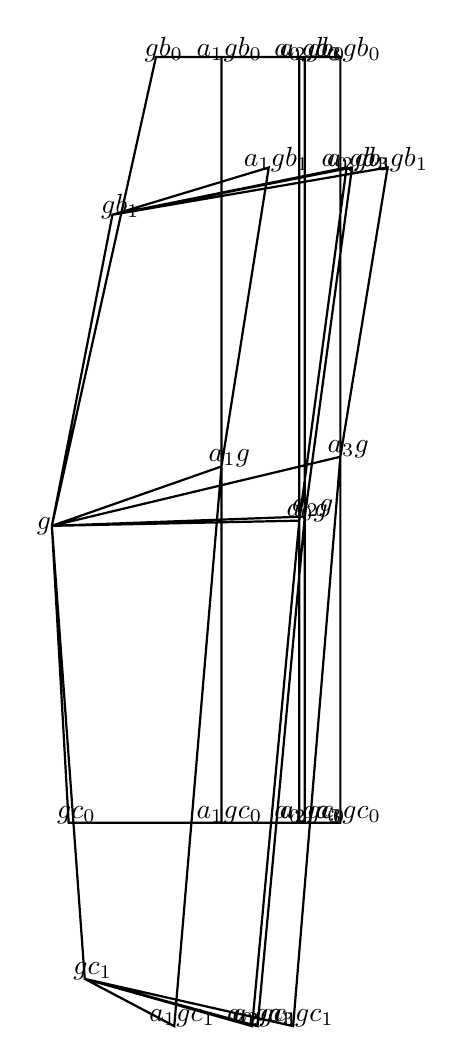
\begin{tikzpicture}
            \draw[thick](0,0)(0,0) -- (1.3217073559081647,5.953492575865221) -- (3.1425689418130816,5.953492575865221) -- (3.1425689418130816,0.06600178113126466) -- (0,0)
(0,0) -- (0.7694892926925494,3.951023551032428) -- (3.7425689418130816,4.5510235510324275) -- (3.1425689418130816,0.06600178113126466) -- (0,0)
(0,0) -- (1.3217073559081647,5.953492575865221) -- (2.1541798877665057,5.953492575865221) -- (2.1541798877665057,0.7543901460937219) -- (0,0)
(0,0) -- (0.7694892926925494,3.951023551032428) -- (2.754179887766506,4.5510235510324275) -- (2.1541798877665057,0.7543901460937219) -- (0,0)
(0,0) -- (1.3217073559081647,5.953492575865221) -- (3.2121317957745203,5.953492575865221) -- (3.2121317957745203,0.11840129664917577) -- (0,0)
(0,0) -- (0.7694892926925494,3.951023551032428) -- (3.8121317957745204,4.5510235510324275) -- (3.2121317957745203,0.11840129664917577) -- (0,0)
(0,0) -- (1.3217073559081647,5.953492575865221) -- (3.6638252190851532,5.953492575865221) -- (3.6638252190851532,0.8775628181022556) -- (0,0)
(0,0) -- (0.7694892926925494,3.951023551032428) -- (4.263825219085153,4.5510235510324275) -- (3.6638252190851532,0.8775628181022556) -- (0,0)
(0,0) -- (0.21317328185556694,-3.7717100698710047) -- (3.1425689418130816,-3.7717100698710047) -- (3.1425689418130816,0.06600178113126466) -- (0,0)
(0,0) -- (0.4179320752205984,-5.753605554729075) -- (2.5425689418130815,-6.353605554729075) -- (3.1425689418130816,0.06600178113126466) -- (0,0)
(0,0) -- (0.21317328185556694,-3.7717100698710047) -- (2.1541798877665057,-3.7717100698710047) -- (2.1541798877665057,0.7543901460937219) -- (0,0)
(0,0) -- (0.4179320752205984,-5.753605554729075) -- (1.5541798877665056,-6.353605554729075) -- (2.1541798877665057,0.7543901460937219) -- (0,0)
(0,0) -- (0.21317328185556694,-3.7717100698710047) -- (3.2121317957745203,-3.7717100698710047) -- (3.2121317957745203,0.11840129664917577) -- (0,0)
(0,0) -- (0.4179320752205984,-5.753605554729075) -- (2.6121317957745203,-6.353605554729075) -- (3.2121317957745203,0.11840129664917577) -- (0,0)
(0,0) -- (0.21317328185556694,-3.7717100698710047) -- (3.6638252190851532,-3.7717100698710047) -- (3.6638252190851532,0.8775628181022556) -- (0,0)
(0,0) -- (0.4179320752205984,-5.753605554729075) -- (3.063825219085153,-6.353605554729075) -- (3.6638252190851532,0.8775628181022556) -- (0,0)
;
\node at (3.2425689418130816,6.053492575865221) {$ a_{ 0  } gb_{ 0 } $};
\node at (3.8425689418130817,4.651023551032427) {$ a_{ 0  } gb_{ 1 } $};
\node at (2.254179887766506,6.053492575865221) {$ a_{ 1  } gb_{ 0 } $};
\node at (2.854179887766506,4.651023551032427) {$ a_{ 1  } gb_{ 1 } $};
\node at (3.3121317957745204,6.053492575865221) {$ a_{ 2  } gb_{ 0 } $};
\node at (3.9121317957745205,4.651023551032427) {$ a_{ 2  } gb_{ 1 } $};
\node at (3.7638252190851533,6.053492575865221) {$ a_{ 3  } gb_{ 0 } $};
\node at (4.363825219085153,4.651023551032427) {$ a_{ 3  } gb_{ 1 } $};
\node at (3.2425689418130816,-3.6717100698710046) {$ a_{ 0  } gc_{ 0 } $};
\node at (2.6425689418130816,-6.253605554729075) {$ a_{ 0  } gc_{ 1 } $};
\node at (2.254179887766506,-3.6717100698710046) {$ a_{ 1  } gc_{ 0 } $};
\node at (1.6541798877665057,-6.253605554729075) {$ a_{ 1  } gc_{ 1 } $};
\node at (3.3121317957745204,-3.6717100698710046) {$ a_{ 2  } gc_{ 0 } $};
\node at (2.7121317957745203,-6.253605554729075) {$ a_{ 2  } gc_{ 1 } $};
\node at (3.7638252190851533,-3.6717100698710046) {$ a_{ 3  } gc_{ 0 } $};
\node at (3.1638252190851532,-6.253605554729075) {$ a_{ 3  } gc_{ 1 } $};
\node at (-0.1,0) {$ g $};
\node at (3.2425689418130816,0.16600178113126468) {$ a_{ 0 }g $};
\node at (2.254179887766506,0.8543901460937219) {$ a_{ 1 }g $};
\node at (3.3121317957745204,0.2184012966491758) {$ a_{ 2 }g $};
\node at (3.7638252190851533,0.9775628181022555) {$ a_{ 3 }g $};
\node at (1.4217073559081648,6.053492575865221) {$ gb_{ 0 } $};
\node at (0.8694892926925494,4.0510235510324275) {$ gb_{ 1 } $};
\node at (0.3131732818555669,-3.6717100698710046) {$ gc_{ 0 } $};
\node at (0.5179320752205984,-5.653605554729076) {$ gc_{ 1 } $};

            \end{tikzpicture}
            \end{center}
            \caption{Square of the complex, with edges $(g,ag), (agb, gb) \in E_A,
            (g,gb), (agb, ag) \in E_B.$ \label{fig:square}
            }
            \end{figure}
 \begin{figure}[H]
            %\label{fig:square}
            \begin{center}
            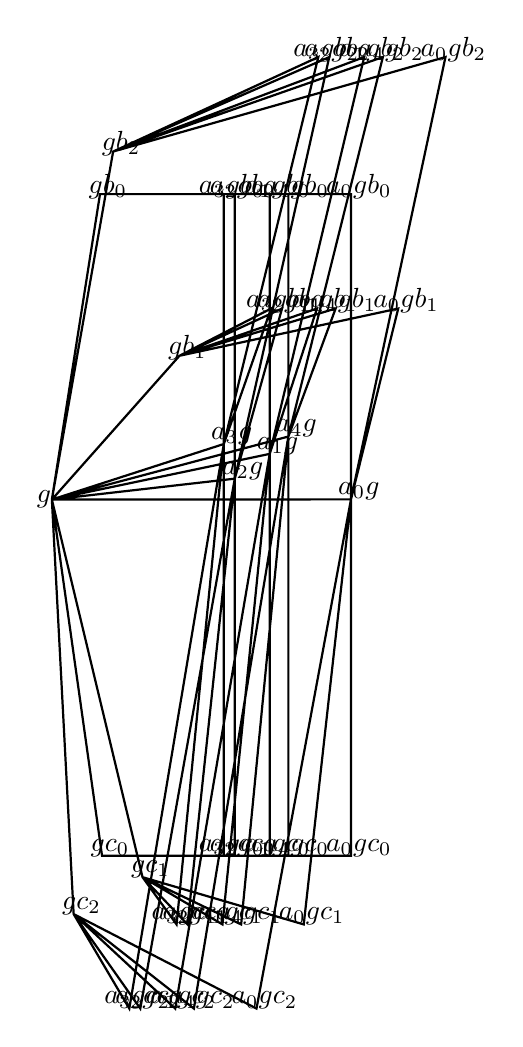
\begin{tikzpicture}
            \draw[thick](0,0)(0,0) -- (0.6112139211145255,3.8788714882011366) -- (3.7986447763994695,3.8788714882011366) -- (3.7986447763994695,0.002431238970634686) -- (0,0)
(0,0) -- (1.6204699753733791,1.8259090185381701) -- (4.398644776399469,2.42590901853817) -- (3.7986447763994695,0.002431238970634686) -- (0,0)
(0,0) -- (0.7779542354290023,4.419591698085448) -- (4.99864477639947,5.619591698085448) -- (3.7986447763994695,0.002431238970634686) -- (0,0)
(0,0) -- (0.6112139211145255,3.8788714882011366) -- (2.7666618481228573,3.8788714882011366) -- (2.7666618481228573,0.579985326486897) -- (0,0)
(0,0) -- (1.6204699753733791,1.8259090185381701) -- (3.3666618481228574,2.42590901853817) -- (2.7666618481228573,0.579985326486897) -- (0,0)
(0,0) -- (0.7779542354290023,4.419591698085448) -- (3.9666618481228575,5.619591698085448) -- (2.7666618481228573,0.579985326486897) -- (0,0)
(0,0) -- (0.6112139211145255,3.8788714882011366) -- (2.322953196654461,3.8788714882011366) -- (2.322953196654461,0.2653773008861262) -- (0,0)
(0,0) -- (1.6204699753733791,1.8259090185381701) -- (2.9229531966544613,2.42590901853817) -- (2.322953196654461,0.2653773008861262) -- (0,0)
(0,0) -- (0.7779542354290023,4.419591698085448) -- (3.522953196654461,5.619591698085448) -- (2.322953196654461,0.2653773008861262) -- (0,0)
(0,0) -- (0.6112139211145255,3.8788714882011366) -- (2.1835723127922133,3.8788714882011366) -- (2.1835723127922133,0.7055553990731505) -- (0,0)
(0,0) -- (1.6204699753733791,1.8259090185381701) -- (2.7835723127922134,2.42590901853817) -- (2.1835723127922133,0.7055553990731505) -- (0,0)
(0,0) -- (0.7779542354290023,4.419591698085448) -- (3.3835723127922135,5.619591698085448) -- (2.1835723127922133,0.7055553990731505) -- (0,0)
(0,0) -- (0.6112139211145255,3.8788714882011366) -- (3.0036844893004946,3.8788714882011366) -- (3.0036844893004946,0.8003895791180177) -- (0,0)
(0,0) -- (1.6204699753733791,1.8259090185381701) -- (3.6036844893004947,2.42590901853817) -- (3.0036844893004946,0.8003895791180177) -- (0,0)
(0,0) -- (0.7779542354290023,4.419591698085448) -- (4.203684489300494,5.619591698085448) -- (3.0036844893004946,0.8003895791180177) -- (0,0)
(0,0) -- (0.6371190685204955,-4.522672272480754) -- (3.7986447763994695,-4.522672272480754) -- (3.7986447763994695,0.002431238970634686) -- (0,0)
(0,0) -- (1.1515684664511405,-4.79574685876479) -- (3.1986447763994694,-5.39574685876479) -- (3.7986447763994695,0.002431238970634686) -- (0,0)
(0,0) -- (0.27645871167780856,-5.2641363676230855) -- (2.5986447763994693,-6.464136367623086) -- (3.7986447763994695,0.002431238970634686) -- (0,0)
(0,0) -- (0.6371190685204955,-4.522672272480754) -- (2.7666618481228573,-4.522672272480754) -- (2.7666618481228573,0.579985326486897) -- (0,0)
(0,0) -- (1.1515684664511405,-4.79574685876479) -- (2.1666618481228572,-5.39574685876479) -- (2.7666618481228573,0.579985326486897) -- (0,0)
(0,0) -- (0.27645871167780856,-5.2641363676230855) -- (1.5666618481228574,-6.464136367623086) -- (2.7666618481228573,0.579985326486897) -- (0,0)
(0,0) -- (0.6371190685204955,-4.522672272480754) -- (2.322953196654461,-4.522672272480754) -- (2.322953196654461,0.2653773008861262) -- (0,0)
(0,0) -- (1.1515684664511405,-4.79574685876479) -- (1.7229531966544611,-5.39574685876479) -- (2.322953196654461,0.2653773008861262) -- (0,0)
(0,0) -- (0.27645871167780856,-5.2641363676230855) -- (1.1229531966544612,-6.464136367623086) -- (2.322953196654461,0.2653773008861262) -- (0,0)
(0,0) -- (0.6371190685204955,-4.522672272480754) -- (2.1835723127922133,-4.522672272480754) -- (2.1835723127922133,0.7055553990731505) -- (0,0)
(0,0) -- (1.1515684664511405,-4.79574685876479) -- (1.5835723127922132,-5.39574685876479) -- (2.1835723127922133,0.7055553990731505) -- (0,0)
(0,0) -- (0.27645871167780856,-5.2641363676230855) -- (0.9835723127922134,-6.464136367623086) -- (2.1835723127922133,0.7055553990731505) -- (0,0)
(0,0) -- (0.6371190685204955,-4.522672272480754) -- (3.0036844893004946,-4.522672272480754) -- (3.0036844893004946,0.8003895791180177) -- (0,0)
(0,0) -- (1.1515684664511405,-4.79574685876479) -- (2.4036844893004945,-5.39574685876479) -- (3.0036844893004946,0.8003895791180177) -- (0,0)
(0,0) -- (0.27645871167780856,-5.2641363676230855) -- (1.8036844893004946,-6.464136367623086) -- (3.0036844893004946,0.8003895791180177) -- (0,0)
;
\node at (3.8986447763994696,3.9788714882011367) {$ a_{ 0  } gb_{ 0 } $};
\node at (4.498644776399469,2.52590901853817) {$ a_{ 0  } gb_{ 1 } $};
\node at (5.098644776399469,5.7195916980854475) {$ a_{ 0  } gb_{ 2 } $};
\node at (2.8666618481228574,3.9788714882011367) {$ a_{ 1  } gb_{ 0 } $};
\node at (3.4666618481228575,2.52590901853817) {$ a_{ 1  } gb_{ 1 } $};
\node at (4.066661848122857,5.7195916980854475) {$ a_{ 1  } gb_{ 2 } $};
\node at (2.4229531966544613,3.9788714882011367) {$ a_{ 2  } gb_{ 0 } $};
\node at (3.0229531966544614,2.52590901853817) {$ a_{ 2  } gb_{ 1 } $};
\node at (3.622953196654461,5.7195916980854475) {$ a_{ 2  } gb_{ 2 } $};
\node at (2.2835723127922134,3.9788714882011367) {$ a_{ 3  } gb_{ 0 } $};
\node at (2.8835723127922135,2.52590901853817) {$ a_{ 3  } gb_{ 1 } $};
\node at (3.4835723127922136,5.7195916980854475) {$ a_{ 3  } gb_{ 2 } $};
\node at (3.1036844893004947,3.9788714882011367) {$ a_{ 4  } gb_{ 0 } $};
\node at (3.7036844893004948,2.52590901853817) {$ a_{ 4  } gb_{ 1 } $};
\node at (4.303684489300494,5.7195916980854475) {$ a_{ 4  } gb_{ 2 } $};
\node at (3.8986447763994696,-4.422672272480755) {$ a_{ 0  } gc_{ 0 } $};
\node at (3.2986447763994695,-5.29574685876479) {$ a_{ 0  } gc_{ 1 } $};
\node at (2.6986447763994694,-6.364136367623086) {$ a_{ 0  } gc_{ 2 } $};
\node at (2.8666618481228574,-4.422672272480755) {$ a_{ 1  } gc_{ 0 } $};
\node at (2.2666618481228573,-5.29574685876479) {$ a_{ 1  } gc_{ 1 } $};
\node at (1.6666618481228574,-6.364136367623086) {$ a_{ 1  } gc_{ 2 } $};
\node at (2.4229531966544613,-4.422672272480755) {$ a_{ 2  } gc_{ 0 } $};
\node at (1.8229531966544612,-5.29574685876479) {$ a_{ 2  } gc_{ 1 } $};
\node at (1.2229531966544613,-6.364136367623086) {$ a_{ 2  } gc_{ 2 } $};
\node at (2.2835723127922134,-4.422672272480755) {$ a_{ 3  } gc_{ 0 } $};
\node at (1.6835723127922133,-5.29574685876479) {$ a_{ 3  } gc_{ 1 } $};
\node at (1.0835723127922134,-6.364136367623086) {$ a_{ 3  } gc_{ 2 } $};
\node at (3.1036844893004947,-4.422672272480755) {$ a_{ 4  } gc_{ 0 } $};
\node at (2.5036844893004946,-5.29574685876479) {$ a_{ 4  } gc_{ 1 } $};
\node at (1.9036844893004947,-6.364136367623086) {$ a_{ 4  } gc_{ 2 } $};
\node at (-0.1,0) {$ g $};
\node at (3.8986447763994696,0.10243123897063469) {$ a_{ 0 }g $};
\node at (2.8666618481228574,0.679985326486897) {$ a_{ 1 }g $};
\node at (2.4229531966544613,0.3653773008861262) {$ a_{ 2 }g $};
\node at (2.2835723127922134,0.8055553990731504) {$ a_{ 3 }g $};
\node at (3.1036844893004947,0.9003895791180176) {$ a_{ 4 }g $};
\node at (0.7112139211145255,3.9788714882011367) {$ gb_{ 0 } $};
\node at (1.7204699753733792,1.9259090185381702) {$ gb_{ 1 } $};
\node at (0.8779542354290023,4.519591698085447) {$ gb_{ 2 } $};
\node at (0.7371190685204955,-4.422672272480755) {$ gc_{ 0 } $};
\node at (1.2515684664511406,-4.695746858764791) {$ gc_{ 1 } $};
\node at (0.37645871167780853,-5.164136367623086) {$ gc_{ 2 } $};

            \end{tikzpicture}
            \end{center}
            \caption{Square of the complex, with edges $(g,ag), (agb, gb) \in E_A,
            (g,gb), (agb, ag) \in E_B.$ \label{fig:square}
            }
            \end{figure}
 \begin{figure}[H]
            %\label{fig:square}
            \begin{center}
            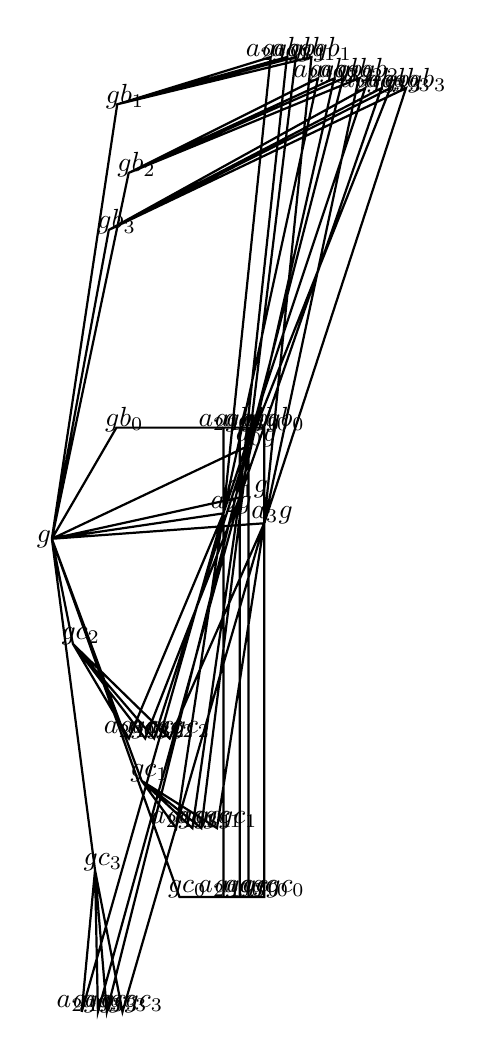
\begin{tikzpicture}
            \draw[thick](0,0)(0,0) -- (0.820038226463184,1.411508199533674) -- (2.4980130502877875,1.411508199533674) -- (2.4980130502877875,1.1818481191903223) -- (0,0)
(0,0) -- (0.8300508700412048,5.517562371839828) -- (3.0980130502877876,6.117562371839828) -- (2.4980130502877875,1.1818481191903223) -- (0,0)
(0,0) -- (0.9754387260455837,4.646462913957862) -- (3.6980130502877877,5.846462913957862) -- (2.4980130502877875,1.1818481191903223) -- (0,0)
(0,0) -- (0.7231240287182401,3.9223002180918694) -- (4.298013050287787,5.722300218091869) -- (2.4980130502877875,1.1818481191903223) -- (0,0)
(0,0) -- (0.820038226463184,1.411508199533674) -- (2.3848461919890855,1.411508199533674) -- (2.3848461919890855,0.5243959032723663) -- (0,0)
(0,0) -- (0.8300508700412048,5.517562371839828) -- (2.9848461919890856,6.117562371839828) -- (2.3848461919890855,0.5243959032723663) -- (0,0)
(0,0) -- (0.9754387260455837,4.646462913957862) -- (3.5848461919890857,5.846462913957862) -- (2.3848461919890855,0.5243959032723663) -- (0,0)
(0,0) -- (0.7231240287182401,3.9223002180918694) -- (4.184846191989085,5.722300218091869) -- (2.3848461919890855,0.5243959032723663) -- (0,0)
(0,0) -- (0.820038226463184,1.411508199533674) -- (2.178704646401566,1.411508199533674) -- (2.178704646401566,0.3228270917718968) -- (0,0)
(0,0) -- (0.8300508700412048,5.517562371839828) -- (2.778704646401566,6.117562371839828) -- (2.178704646401566,0.3228270917718968) -- (0,0)
(0,0) -- (0.9754387260455837,4.646462913957862) -- (3.378704646401566,5.846462913957862) -- (2.178704646401566,0.3228270917718968) -- (0,0)
(0,0) -- (0.7231240287182401,3.9223002180918694) -- (3.9787046464015656,5.722300218091869) -- (2.178704646401566,0.3228270917718968) -- (0,0)
(0,0) -- (0.820038226463184,1.411508199533674) -- (2.696752889025511,1.411508199533674) -- (2.696752889025511,0.19686582437496236) -- (0,0)
(0,0) -- (0.8300508700412048,5.517562371839828) -- (3.296752889025511,6.117562371839828) -- (2.696752889025511,0.19686582437496236) -- (0,0)
(0,0) -- (0.9754387260455837,4.646462913957862) -- (3.896752889025511,5.846462913957862) -- (2.696752889025511,0.19686582437496236) -- (0,0)
(0,0) -- (0.7231240287182401,3.9223002180918694) -- (4.496752889025511,5.722300218091869) -- (2.696752889025511,0.19686582437496236) -- (0,0)
(0,0) -- (1.6205123550233942,-4.549329084043638) -- (2.4980130502877875,-4.549329084043638) -- (2.4980130502877875,1.1818481191903223) -- (0,0)
(0,0) -- (1.1407595631947194,-3.074380254446017) -- (1.8980130502877874,-3.674380254446017) -- (2.4980130502877875,1.1818481191903223) -- (0,0)
(0,0) -- (0.26751524536260973,-1.3356051911295816) -- (1.2980130502877876,-2.535605191129582) -- (2.4980130502877875,1.1818481191903223) -- (0,0)
(0,0) -- (0.5482102742795785,-4.207780579538341) -- (0.6980130502877877,-6.007780579538341) -- (2.4980130502877875,1.1818481191903223) -- (0,0)
(0,0) -- (1.6205123550233942,-4.549329084043638) -- (2.3848461919890855,-4.549329084043638) -- (2.3848461919890855,0.5243959032723663) -- (0,0)
(0,0) -- (1.1407595631947194,-3.074380254446017) -- (1.7848461919890855,-3.674380254446017) -- (2.3848461919890855,0.5243959032723663) -- (0,0)
(0,0) -- (0.26751524536260973,-1.3356051911295816) -- (1.1848461919890856,-2.535605191129582) -- (2.3848461919890855,0.5243959032723663) -- (0,0)
(0,0) -- (0.5482102742795785,-4.207780579538341) -- (0.5848461919890857,-6.007780579538341) -- (2.3848461919890855,0.5243959032723663) -- (0,0)
(0,0) -- (1.6205123550233942,-4.549329084043638) -- (2.178704646401566,-4.549329084043638) -- (2.178704646401566,0.3228270917718968) -- (0,0)
(0,0) -- (1.1407595631947194,-3.074380254446017) -- (1.5787046464015657,-3.674380254446017) -- (2.178704646401566,0.3228270917718968) -- (0,0)
(0,0) -- (0.26751524536260973,-1.3356051911295816) -- (0.9787046464015658,-2.535605191129582) -- (2.178704646401566,0.3228270917718968) -- (0,0)
(0,0) -- (0.5482102742795785,-4.207780579538341) -- (0.378704646401566,-6.007780579538341) -- (2.178704646401566,0.3228270917718968) -- (0,0)
(0,0) -- (1.6205123550233942,-4.549329084043638) -- (2.696752889025511,-4.549329084043638) -- (2.696752889025511,0.19686582437496236) -- (0,0)
(0,0) -- (1.1407595631947194,-3.074380254446017) -- (2.096752889025511,-3.674380254446017) -- (2.696752889025511,0.19686582437496236) -- (0,0)
(0,0) -- (0.26751524536260973,-1.3356051911295816) -- (1.496752889025511,-2.535605191129582) -- (2.696752889025511,0.19686582437496236) -- (0,0)
(0,0) -- (0.5482102742795785,-4.207780579538341) -- (0.8967528890255112,-6.007780579538341) -- (2.696752889025511,0.19686582437496236) -- (0,0)
;
\node at (2.5980130502877876,1.511508199533674) {$ a_{ 0  } gb_{ 0 } $};
\node at (3.1980130502877877,6.217562371839827) {$ a_{ 0  } gb_{ 1 } $};
\node at (3.798013050287788,5.946462913957862) {$ a_{ 0  } gb_{ 2 } $};
\node at (4.398013050287787,5.822300218091868) {$ a_{ 0  } gb_{ 3 } $};
\node at (2.4848461919890856,1.511508199533674) {$ a_{ 1  } gb_{ 0 } $};
\node at (3.0848461919890857,6.217562371839827) {$ a_{ 1  } gb_{ 1 } $};
\node at (3.684846191989086,5.946462913957862) {$ a_{ 1  } gb_{ 2 } $};
\node at (4.284846191989085,5.822300218091868) {$ a_{ 1  } gb_{ 3 } $};
\node at (2.278704646401566,1.511508199533674) {$ a_{ 2  } gb_{ 0 } $};
\node at (2.878704646401566,6.217562371839827) {$ a_{ 2  } gb_{ 1 } $};
\node at (3.478704646401566,5.946462913957862) {$ a_{ 2  } gb_{ 2 } $};
\node at (4.078704646401565,5.822300218091868) {$ a_{ 2  } gb_{ 3 } $};
\node at (2.796752889025511,1.511508199533674) {$ a_{ 3  } gb_{ 0 } $};
\node at (3.396752889025511,6.217562371839827) {$ a_{ 3  } gb_{ 1 } $};
\node at (3.9967528890255113,5.946462913957862) {$ a_{ 3  } gb_{ 2 } $};
\node at (4.5967528890255105,5.822300218091868) {$ a_{ 3  } gb_{ 3 } $};
\node at (2.5980130502877876,-4.449329084043638) {$ a_{ 0  } gc_{ 0 } $};
\node at (1.9980130502877875,-3.574380254446017) {$ a_{ 0  } gc_{ 1 } $};
\node at (1.3980130502877877,-2.4356051911295817) {$ a_{ 0  } gc_{ 2 } $};
\node at (0.7980130502877877,-5.907780579538342) {$ a_{ 0  } gc_{ 3 } $};
\node at (2.4848461919890856,-4.449329084043638) {$ a_{ 1  } gc_{ 0 } $};
\node at (1.8848461919890855,-3.574380254446017) {$ a_{ 1  } gc_{ 1 } $};
\node at (1.2848461919890857,-2.4356051911295817) {$ a_{ 1  } gc_{ 2 } $};
\node at (0.6848461919890857,-5.907780579538342) {$ a_{ 1  } gc_{ 3 } $};
\node at (2.278704646401566,-4.449329084043638) {$ a_{ 2  } gc_{ 0 } $};
\node at (1.6787046464015658,-3.574380254446017) {$ a_{ 2  } gc_{ 1 } $};
\node at (1.078704646401566,-2.4356051911295817) {$ a_{ 2  } gc_{ 2 } $};
\node at (0.47870464640156596,-5.907780579538342) {$ a_{ 2  } gc_{ 3 } $};
\node at (2.796752889025511,-4.449329084043638) {$ a_{ 3  } gc_{ 0 } $};
\node at (2.196752889025511,-3.574380254446017) {$ a_{ 3  } gc_{ 1 } $};
\node at (1.5967528890255112,-2.4356051911295817) {$ a_{ 3  } gc_{ 2 } $};
\node at (0.9967528890255112,-5.907780579538342) {$ a_{ 3  } gc_{ 3 } $};
\node at (-0.1,0) {$ g $};
\node at (2.5980130502877876,1.2818481191903224) {$ a_{ 0 }g $};
\node at (2.4848461919890856,0.6243959032723663) {$ a_{ 1 }g $};
\node at (2.278704646401566,0.4228270917718968) {$ a_{ 2 }g $};
\node at (2.796752889025511,0.29686582437496234) {$ a_{ 3 }g $};
\node at (0.920038226463184,1.511508199533674) {$ gb_{ 0 } $};
\node at (0.9300508700412048,5.617562371839828) {$ gb_{ 1 } $};
\node at (1.0754387260455838,4.746462913957862) {$ gb_{ 2 } $};
\node at (0.8231240287182401,4.022300218091869) {$ gb_{ 3 } $};
\node at (1.7205123550233943,-4.449329084043638) {$ gc_{ 0 } $};
\node at (1.2407595631947195,-2.9743802544460167) {$ gc_{ 1 } $};
\node at (0.3675152453626097,-1.2356051911295816) {$ gc_{ 2 } $};
\node at (0.6482102742795784,-4.107780579538342) {$ gc_{ 3 } $};

            \end{tikzpicture}
            \end{center}
            \caption{Square of the complex, with edges $(g,ag), (agb, gb) \in E_A,
            (g,gb), (agb, ag) \in E_B.$ \label{fig:square}
            }
            \end{figure}
 
\end{multicols*}
  % \printbibliography 
\end{document}

 